\documentclass[pdftex,11pt,a4paper]{article}
\usepackage{anysize}
\marginsize{2.5cm}{2.5cm}{1.5cm}{1.5cm}
\usepackage[pdftex]{graphicx}
\usepackage{wrapfig}
\usepackage{url}
\usepackage{listings}
\usepackage{color}
\usepackage{textcomp}

\lstset{
	backgroundcolor=\color{lbcolor},
	tabsize=2,
	language=java,
	numbers=left,
	numbersep=5pt,
        basicstyle=\scriptsize,
        upquote=true,
        aboveskip={1.5\baselineskip},
        columns=fixed,
        showstringspaces=false,
        extendedchars=true,
        breaklines=true,
        prebreak = \raisebox{0ex}[0ex][0ex]{\ensuremath{\hookleftarrow}},
        showtabs=false,
        showspaces=false,
        showstringspaces=false,
        identifierstyle=\ttfamily,
        keywordstyle=\color[rgb]{0,0,1},
        commentstyle=\color[rgb]{0.133,0.545,0.133},
        stringstyle=\color[rgb]{0.627,0.126,0.941},
}



\definecolor{listinggray}{gray}{0.9}
\definecolor{lbcolor}{rgb}{0.9,0.9,0.9}
\linespread{1.2}
\setlength{\parindent}{0pt}
\setlength{\parskip}{1ex plus 0.8ex minus 0.2ex}

\usepackage{fancyhdr}

\pagestyle{fancy}
\lhead{\footnotesize {Systems Architecture Project} }
\rhead{\footnotesize {Client orders framework} }

\renewcommand\headheight{24pt}
\renewcommand\footrulewidth{0.4pt}

\clearpage
\newcommand{\HRule}{\rule{\linewidth}{0.5mm}}

\author{John \textsc{Flanagan} 0702009 \& Marcin \textsc{Wrzeszcz} 0726753 }
\title{TITLE GOES HERE}
\date{\today}

\begin{document}

\begin{titlepage}
 
\begin{center}
 
 
% Upper part of the page
%\includegraphics[width=0.8\textwidth]{images/logo.pdf}\\[3.5cm]
 
%\textsc{\LARGE Ubiquitous Merchant Legerity}\\[1.5cm]
 
\textsc{\LARGE Assignment 1}\\[3.5cm]
 
 
% Title
\HRule \\[0.6cm]
{ \huge \bfseries Retail software framework}\\Concurrent Architecture\\[0.4cm]
 
\HRule \\[4.0cm]
 {\large \today}\\[9.0cm]

\begin{flushleft} \large
\emph{Module:}\\
CS4135 Software Architecture
\\[0.4cm]
\emph{Authors:}\\
Marcin \textsc{Wrzeszcz} 0726753 \& John \textsc{Flanagan} 0702009
\end{flushleft}

 
\vfill
 

 
\end{center}
 
\end{titlepage}



\pagebreak

\tableofcontents
\pagebreak

\section{Concurrency}
Modern computing environments typically offer upwards of four logical execution cores and in many cases much more. This recent increase in the number processing cores comes as a result of the major manufacturers reaching the limits of clock speed, which is largely due to thermal, manufacturing and power efficiency issues. This has pushed manufactures to concentrate on increasing performance of the individual core by making it more power efficient, piplining operations and better branch prediction. While increasing the number of cores on a die enabling the processors to be scaled-outwards instead of the traditional upwards clock speed scaling. While this description is grossly oversimplified it provides a basic grounding to our understanding of why concurrency is important in modern software applications and some of the issues that arise when performing tasks in parallel. 

For any reasonable sized software system it is important to incorporate a threaded architecture, to enable efficient usage of resources and making the system more responsive. But simply adding threads everywhere is not a guarantee to making a system performant, in some cases the overhead from the setup and tear-down of a thread or the extra context switching may in fact cause a degradation in performance. So the decision to parallelise a module must be backed with performance figures from typical workloads as with any sort of performance tuning.

All modern programming languages today as a matter of course include support for at least one form of threading, with external threading libraries supporting parallelisation across more exotic architectures such as the current trend in utilising GPU cores for floating point arithmetic. 

Writing well threaded code is generally regarded as being quite difficult to do well, there are many issues that arise from concurrent streams of execution. Simple tasks such as reading from and writing to memory becomes difficult with problems of synchronisation between threads when accessing particular resources which in turn can lead to dead lock issues starvation of these resources.


\pagebreak
\section{Results}
The module of the system that was selected for the addition of concurrency was the ComputerAssembler with utilised the builder pattern. Below you can see the modifications made to the assembler class in order to facilitate threading.

\subsection{Timings}
\begin{center}
	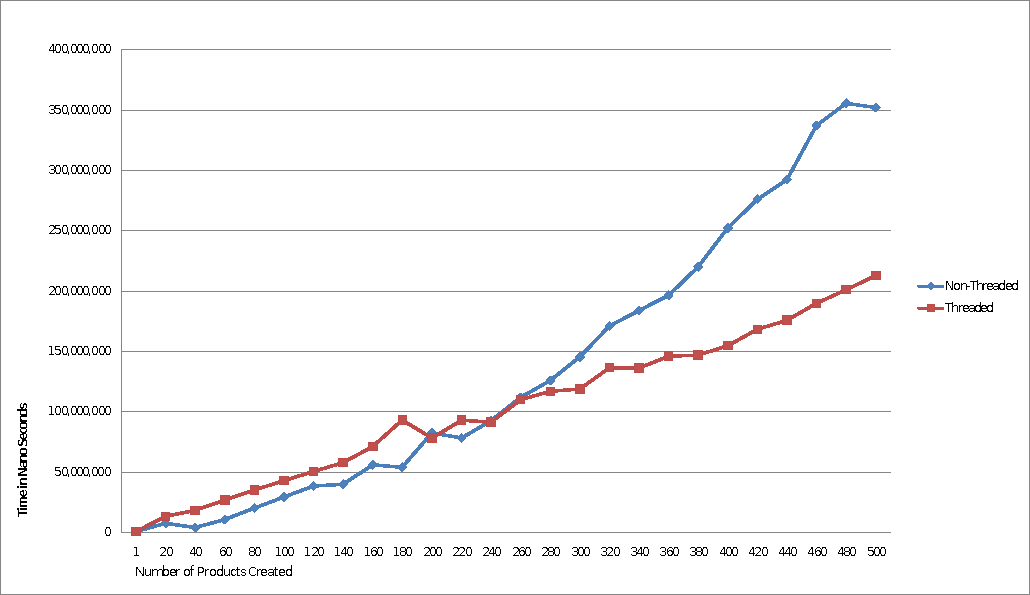
\includegraphics[scale=0.9,angle=0]{graph.pdf}
\end{center}
From viewing the graph its quite clear to see that when less than 200 products being created in our test environment there is a quite clear performance win for a single threaded implementation. But after passing 260 products in our environment a threaded solution is clearly beneficial. These results are compiled as averages over multiple runs and the tests were run on a modern architecture offering up to 8 virtual threads in hardware.
\pagebreak
\subsection{Code}
\lstinputlisting{code/nonthreaded.java}
Single threaded
\lstinputlisting{code/threaded.java}
Multi-threaded

\pagebreak





\end{document}
